\documentclass[10pt,a4paper]{article}
\usepackage[utf8]{inputenc}
\usepackage[german]{babel}
\usepackage[T1]{fontenc}
\usepackage{fullpage}
\usepackage{amssymb}
\usepackage{listings}
\usepackage{caption}
\usepackage{color}
\usepackage{amsmath}
\usepackage{graphicx}
\usepackage[backend=bibtex]{biblatex}
\usepackage{hyperref}
% Bibliography
\addbibresource{bibliography.bib}
% Code snippet style
% Python colored syntax highlighting
\usepackage{listings}
\usepackage{color}
\usepackage{amsmath}
\definecolor{dark-gray}{RGB}{135,135,135}
\definecolor{light-blue}{RGB}{102,178,255}
\definecolor{light-orchid}{RGB}{210,120,210}
\lstdefinelanguage{python-color}{
 morekeywords={and, as, assert, break, class, continue, def, del, elif, else, except, exec, finally, for, from, global, if, import, in, is, lambda, not, or, pass, print, raise, return, try, while, with, yield, None, True, False, import},
 ndkeywords={self},
 keywordstyle=\color{blue}\bfseries,
 ndkeywordstyle=\color{light-orchid}\bfseries,
 sensitive=false,
 identifierstyle=\color{black},
 basicstyle=\sffamily ,
 morecomment=[l]{\#},
 morecomment=[s]{/*}{*/},
 morecomment=[s]{"""}{"""},
 morecomment=[l][\color{light-blue}]{@},
 morecomment=[s][\color{light-blue}]{"}{"},
 commentstyle=\itshape\color{dark-gray},
 stringstyle=\color{red}\ttfamily,
 tabsize=2,
 columns=fullflexible,
 literate={^}{{$\mspace{-3mu}\hat{\quad}\mspace{-5mu}$}}1
 {<}{$<$}2 
 {>}{$>$}2 
 {<:}{{$<\mspace{-3mu}:$}}2 
 {:>}{{$:\mspace{-3mu}>$}}2
 {+}{$+$ }2 
 {++}{{$+\mspace{-8mu}+$ }}2
 {\~}{{$\mspace{-3mu}\tilde{\quad}\mspace{-3mu}$}}1
 {\~}{$\sim$}1
 {__}{\underline{\hspace{0.5cm}}}1
 {*}{${}^{\ast}$}1 
 {.}{$\mspace{1mu}.\mspace{1mu}$}1
}
\lstset{language=python-color}
\lstset{framexleftmargin=5pt, framextopmargin=5pt, framexbottommargin=5pt, frame=tb, framerule=0pt}
\definecolor{grey}{rgb}{0.9,0.9,0.9}
%\newcounter{nalg}[section] % defines algorithm counter for chapter-level
%\renewcommand{\thenalg}{\thechapter .\arabic{nalg}} %defines appearance of the algorithm counter
%\DeclareCaptionLabelFormat{algocaption}{Algorithm \thenalg} % defines a new caption label as Algorithm x.y

\lstnewenvironment{algorithm}[1][] %defines the algorithm listing environment
{   
    %\refstepcounter{nalg} %increments algorithm number
    %\captionsetup{labelformat=algocaption,labelsep=colon} %defines the caption setup for: it ises label format as the declared caption label above and makes label and caption text to be separated by a ':'
    \lstset{ %this is the stype
        mathescape=true,
        keywordstyle=\color{black}\bfseries\em,
        keywords={,input, output, return, datatype, function, in, if, else, foreach, while, begin, end, for, endfor, from, to, do, loop, print, }, %add the keywords you want, or load a language as Rubens explains in his comment above.        
        #1 % this is to add specific settings to an usage of this environment (for instnce, the caption and referable label)
    }
}
{}

\setlength{\parindent}{0pt}
\setlength{\columnsep}{0.5cm}

\title{Teil II:\\Ausarbeitung zum WEP-Protokoll}
\author{Lukas Jung, Marc Narres-Schulz, Oliver Sänger, Tobias Zeimetz}


\begin{document}
\maketitle
\tableofcontents
\newpage

\section{Einführung}
Bei der vorliegenden Arbeit handelt es sich um ein Protokoll über eine Teilaufgabe im \glqq Hackerpraktikum\grqq. Die erste Aufgabe bestand darin, sich in WEP und damit auch in RC4 einzuarbeiten. Hauptbestandteil für das Verständnis von WEP und RC4 waren die Artikel \glqq Attacks on the RC4 stream cipher\grqq \cite{Kle08}, \glqq Breaking 104 bit WEP in less than 60 seconds\grqq \cite{TWP07}\ und \glqq Intercepting Mobile Communications: The Insecurity of 802.11\grqq \cite{BGW01}.

Anschließend sollte eine Test-Umgebung und der Angriff nach Klein implementiert werden. Diese Testumgebung war eine programmierte Simulation der RC4-Stromchiffre. Die Testumgebung wurde in Python programmiert und lieferte als Ergebnis paare aus Initialisierungsvektoren (IV) und Stromchiffren. Dass Ziel bei dem Angriff nach Klein war es, den Hauptschlüssel zu berechnen und somit die Verschlüsselung zu brechen. 

Die letzte Aufgabe dieses Abschnitts im Praktikum bestand darin, den Hauptschlüssel eines auf WEP konfigurierten Routers zu berechnen. Wie in der ersten Aufgabe bereits implementiert, eigenen sich Paare von IV und Schlüsselstrom sehr gut. Um das Auftreten von ARP-Paketen zu erhöhen sollte eine Technik namens \glqq re-injection\grqq \ verwendet werden.  Dazu sollten die Tools \glqq aireplay-ng\grqq \ und \glqq airodump-ng\grqq \ verwendet werden.

Wie bereits erwähnt bestand die letzte Aufgabe darin, aus den ARP-Paketen Paare von IV und und Schlüsselstrom zu berechnen und dadurch den Angriff von Klein auszuführen. Der Angriff lieferte als Ergebnis den Hauptschlüssel und somit wurde die Verschlüsselung von WEP gebrochen.

Das Protokoll besteht aus drei Abschnitten. Der erste Abschnitt dreht sich um die Verschlüsselung und wie diese Funktion. Dort wird genauer erläutert wie die RC4-Stromchiffre funktioniert, wie das WEP-Protokoll arbeitet und was unter den einzelnen Begrifflichkeiten zu verstehen ist. Anschließend wird im Detail auf den ausgeführten Angriff eingegangen. Dieser Abschnitt unterteilt sich zum einen in den Angriff nach Klein und anschließend folgt eine Verbesserung des Angriffs. \textbf{Der letzte Abschnitt.... muss noch ausformuliert werden...}
%TODO

\section{Grundlagen der Verschlüsselung}
Zuerst folgt eine Einführung in die Verschlüsselung die verwendet wird. Dazu unterteilt sich dieses Kapitel in zwei Abschnitte; wie ist die Funktionsweise der RC4-Stromchiffre und des WEP-Protokolls. Die hier verwendete Literatur waren die Artikel \glqq Attacks on the RC4 stream cipher\grqq \cite{Kle08}, \glqq Breaking 104 bit WEP in less than 60 seconds\grqq \cite{TWP07}\ und \glqq Intercepting Mobile Communications: The Insecurity of 802.11\grqq \cite{BGW01}. Zuerst folgt eine Erklärung zum Verfahren der RC4-Stromchiffre und im Anschluss folgt eine Erklärung zum WEP-Protokoll.

\subsection{RC4-Stromchiffre}
Der Algorithmus zu RC4 wurde 1987 von Ron Rivest entwickelt und besteht aus zwei Teilen. Der erste Teil ist das \glqq key scheduling\grqq \ und der zweite Teil ist eine \glqq pseudo random generation\grqq. Der RC4-Algorithmus bekommt zwei Übergabeparameter. Der erste Parameter ist ein zufällig gewählter Initialisierungsvektor (IV). Beim IV handelt es sich um ein Feld mit Einträgen aus $\mathbb{Z}_n$ und $n \in \mathbb{N}$. Beim zweiten Parameter $k$ handelt es sich um den \glqq main key\grqq. Die Konkatenation von IV und \glqq main key\grqq \ bilden den session key. Der session key wird meist als ein ein Feld $K$ implementiert. Da in WEP der IV immer vorne an die verschlüsselte Nachricht angefügt wird, hat der session key folgende Form:
\begin{quote}
	session key = IV || main key
\end{quote}
Das Symbol || stellt den Operator für die Konkatenation dar. Die länge von $k$ und die Größe des IVs sind Abhängig vom gewählten Modus. Bei einer 64-Bit-Verschlüsselung hat der IV eine Größe von 24 Bit und der main key ist 40 Bit groß. Wählt man die 128-Bit-Verschlüsselung so ergibt für den main key eine Größe von 104 Bit. Die Größe des IVs bleib unverändert bei 24 Bit. Somit ergibt sich die Größe $l_K$ des session keys wie folgt:
\begin{quote}
	| K | = | IV | + | k |
\end{quote}
Die maximale Größe von $l_K$ beträgt $n$, liegt jedoch typischerweise zwischen 5 und 128 Bit.

In der ersten Phase des RC4-Algorithmus, der key scheduling phase, wird eine initiale Permutation mit Hilfe des session keys $K$ erzeugt. Die erste Phase lässt sich wie folgt darstellen:\\
\begin{center}
\hspace{5pt}
\begin{minipage}[t]{.35\textwidth}
\begin{algorithm}
{initialization}
for i from 0 to n-1 do
    S[i] := i
end for
j := 0
{generate a random permutation}
for i from 0 to n-1 do
    j := (j+S[i]+K[i mod l]) mod n
    Swap S[i] and S[j]
end for
\end{algorithm}
\end{minipage}\hspace{0.4cm}
\begin{minipage}[t]{.60\textwidth}
  \begin{lstlisting}
def keyScheduling(sessionKey=bytearray(), n=256):
	# initialization
	sBox = []
	for i in range(n):
   		sBox.append(i)
   		sBox = bytearray(sBox)

   	i,j = 0,0
   	# generate a random permutation
   	for i in range(n):
     	j = (j + sBox[i] + sessionKey[i % len(sessionKey)]) % n
    	sBox[i], sBox[j] = sBox[j], sBox[i]

	return sBox
\end{lstlisting}
\end{minipage}
\end{center}

Bei der key scheduling phase wird eine Substitutionsbox (S-Box) verwendet. Diese wird zu beginn mit Werten aus 0 bis $n-1$ aufsteigend gefüllt. Die S-Box wird aus dem geheimen Schlüssel berechnet und später zur Berechnung der Stromchiffre verwendet. In jedem Schritt der For-Schleife werden zwei Einträge der S-Box vertauscht um eine zufällige Permutation zu erzeugen. 

Nachdem die key scheduling phase eine zufällige S-Box generiert hat, beginnt die zweite Phase des RC4-Algorithmus. In dieser Phase wird eine Zufallsfolge, auch Stromchiffre genannt, erstellt. Der Algorithmus dazu gestalltet sich wie folgt:
\begin{center}
\hspace{5pt}
\begin{minipage}[t]{.35\textwidth}
\begin{algorithm}
{initialization}
i := 0
j := 0
{generate pseudo random sequence}
loop
    i := (i + 1) mod n
    j := (j + S[i]) mod n
    Swap S[i] and S[j]
    k := (S[i] + S[j]) mod n
    print S[k]
end loop
\end{algorithm}
\end{minipage}\hspace{0.4cm}
\begin{minipage}[t]{.60\textwidth}
\begin{lstlisting}
def pseudoRandomGenerator(sBox=bytearray(),n=256):
   	# initialization
	i,j = 0,0

	# generate pseudo random sequence
	while True:
   		i = (i + 1) % n
   		j = (j + sBox[i]) % n
   		sBox[i], sBox[j] = sBox[j], sBox[i]
   		k = (sBox[i] + sBox[j]) % n

   		yield bytes([sBox[k]])
\end{lstlisting}
\end{minipage}
\end{center}
Hierbei handelt es sich um den Hauptteil des RC4-Algorithmus.  Der pseudo random generator startet mit dem permutierten Array $sBox$, dass in der key scheduling phase generiert wurde. Anschließend wird ein Index $j$ mit Hilfe der zufällig permutierten S-Box gewählt und zwei Einträge ($sBox[i]$ und $sBox[j]$) werden wie bereits in der key scheduling phase vertauscht. Der nächste Schritt besteht darin einen Index $k$ zu ermitteln, welcher aus den addierten Werten aus der S-Box bestehen. Durch den anschließenden Modulo-Operator wird sichergestellt, dass es sich um Werte aus dem Zahlenraum $\mathbb{Z}_n$ handelt. Der pseudo random generator erstellt somit in jedem Schritt ein Byte, mit einem Wert zwischen $0$ bis $n-1$ als Ausgabe.

\subsection{WEP}
Wired Equivalent Privacy (WEP) ist das ehemalige Standard-Verschlüsselungsprotokoll für WLAN. Das Protokoll wurde dazu verwendet um die Vertraulichkeit und Integrität einer Nachricht sicherzustellen. Die Verschlüsselung unter WEP gestaltet sich wie folgt:
$$
C = (M || c(M)) \oplus RC4(v,k)
$$
Zuerst wird über eine Nachricht $M$ eine Prüfsumme $c(M)$ gebildet. Anschließend wird die Nachricht $M$ mit $c(M)$ konkateniert in der Form $(M || c(M))$. Der nächste Schritt besteht darin den RC4-Algorithmus aufzurufen und so viele zufällige Bytes zu produzieren wie der Term $(M || c(M))$ besitzt. Bei den Variablen die der RC4-Funktion übergeben werden, handelt es sich zum einen um den Initialisierungsvektor $v$ und den main key $k$.

Der letzte Schritt besteht darin die zufällige Bytefolge $RC4(v,k)$ und den Term $(M || c(M)$ mittels XOR zu verrechnen. Dadurch entsteht eine Vernamchiffre $C$ die nur bei Kenntnis von $v$ und $k$ (und letztendlich $RC4(v,k)$) entschlüsselt werden kann.

Über das Netzwerk werden durch den Router Nachrichten verschickt, welche die Form $v || C$ besitzen. Der Initialisierungsvektor wird dabei vorne and die Vernamchiffre konkateniert. Da die Länge des Initialisierungsvektors $v$ bekannt ist, kann der Empfänger der Nachrichten diesen \glqq abschneiden\grqq\ und durch Kenntnis des main keys $k$ die Stromchiffre $RC4(v,k)$ erzeugen. Anschließend kann durch $RC4(v,k) \oplus C$ die Chiffre $C$ entschlüsselt werden.

Durch die Prüfsumme $c(M)$ ist der Empfänger außerdem in der Lage, die Integrität der eigentlichen Nachricht $M$ zu gewährleisten. 

\section{Der Angriff}
%TODO Anpassen
In diesem Abschnitt werden die verschiedenen Angriffe die wir in den Aufgaben 2 bis 4 durchführen sollten genauer dargelegt. Der erste Abschnitt handelt darüber wie Kleins Angriff auf den RC4-Algorithmus unter einer \glqq simulierten Umgebung\grqq \ getestet wurde. Anschließend wird darauf eingegangen wie man das Auftreten von ARP-Paketen  mit Hilfe einer Technik namens \glqq re-injection\grqq \ erhöht. Danach werden aus diesen Paketen Paare von IV und Schlüsselstrom extrahiert und der Angriff von Klein wird auf diese Daten angewendet. Abschließend wird erläutert wie man den Angriff deutlich effizienter machen kann. Im Folgenden wird größtenteils die Notation aus dem Papier \cite[Kapitel 3.1]{TWP07} verwendet.

\subsection{Schwächen in RC4}
%TODO Auf Korrelation in RC4 PRNG eingehen(Klein paper, sowie andere paper kurz zusammenfassen), auf Besonderheiten unserer situation eingehen (iv vorne,...) 
Die von RC4 erzeugte Pseudosufallssequenz (=PZS) unterscheidet sich in einigen Punkten von einer echten Zufallsfolge. Die Summe der letzten Bits in Schritt t und t+2 korreliert gegen 1.
J.Dj. Golic kam zu dem Schluss, dass $2^40$ Bytes von der RC4-PZS unterscheidbar sind zu einer echten Zufallssequenz.
Weitere Untersuchungen von S.R. Fluhrer und D.A. McGrew haben beweisen, das die gemeinsame WK von zwei aufeinander folgenden Bytes sich signifikant von einer Zufallsfolge unterscheiden. Im Idealfall besteht ein Schlüssel aus n unabhägig, identischen und gleichverteilten Elementen aus Z/nZ und gerneriert $n^n$ gleichwahrscheinliche Schlüssel. Jedoch ist $n!$ kein Teiler von $n^n$. Daher muss sich die Verteilung der initialen Permutation von einer Gleichverteilung unterscheiden. (Siehe Studie von I.Mironov)
Für das weitere Vorgehen ist jedoch folgende Schwachstelle wichtig:\\
Das erste Byte der PZS ist nicht wirklich zufällig. Der Angriff von S. Fluhrer, I. Martin und A. Shamir nimmt an, dass der Initialisierungsvektor vor dem Hauptschlüssel steht und die ersten zwei Bytes die Form $(b,n-1)$ haben, wobei $b$ das Byte des Hauptschlüssel ist, welches rekonstruiert werden soll. Wenn ein Angreifer keine Chance hat den Initialisierungsverktor zu beeinflussen, muss er warten, bis der initialiserungsverktor die gewünschte Form annimmt. Die ist in druchschnittlich eine aus $n^2$ Situngen der Fall. Die Authoren zeigen, dass dieser Angriff auf WEP angewendet warden kann.
Es wird festgestellt, dass eine starke Korrelation zwischen den beobachtbaren und abfangbaren Werten der S-Box $i, S[k]$ und den internen Werten von $j, S[j]$ und $S[i]$ besteht.
\subsection{Angriff von Klein}\label{ssec:klein}
Der Angriff von Klein nutzt nun die oben beschriebene Schwäche von RC4 aus. Wir betrachten die Permutation in der Key-Scheduling-Phase.\\
Hier sieht man leicht, nach dem ersten Schritt gilt für Bytes des Schlüssels K und Werte der S-Box S:
\begin{center}
$ j = 0+0+K[0] = K[0] $\\
$\Rightarrow S[0] \textit{ wird vertauscht mit }  S[K[0]] $\\
\end{center}
So lässt sich die zweite Runde (mit Wahrscheinlichkeit $1 - (1/n)$ ebenfalls rekonstruieren:
\begin{center}
$ j = K[0] + 1 + K[1]$\\  
$\Rightarrow S[1] \textit{ wird vertauscht mit } S[ K[0] + 1 + K[1] ] $ ( $K[0] + 1 + K[1]$ ) wird im Weiteren mit  $t$ bezeichnet.\\
\end{center}
Wir wissen nun, dass für ein festes $K[0]$ der Wert $t$ und $S[1]$ sich aus $K[1]$ berechnen lassen.
In den weiteren Schritten der Key-Sheduling-Phase wird $S[1]$ nicht mehr geändert, sofern $j$ nie den Wert 1 annimmt.
Die Wahrscheinlickkeit, dass dies in einem Schritt dennoch passiert liegt bei $1 - (1/n)$ falls der SessionKey die Länge n hat.
Sind alle Keybytes von einander unabhängig, folgt $S[1]$ wird mit der Wahrscheinlichkeit $(1-(1/n))^{n-2} \approx 1/e$ nicht verändert.\\
Nun wissen wir Folgendes:\\
Der Wert von $S[1]$ ist zu Beginn des RC4-PZG $t$. Wobei $t$ mit Wahrscheinlichkeit $(1/e)$ nur von $K[0]$ und $K[1]$ abhängt. Somit kann das in der Arbeit von Klein hergeleitete Theorem 1 \cite{Kle08} benutzt werden um $t$ aus der beobachteten RC4-PZS zu erhalten.\\
Dazu schauen wir uns die Generierung des ersten Pseudozufall-Bytes (PZB) an:\\
Zuerst wird $i$ auf $1$ gesetzt. Daher werden $S[1]$ und $S[j]$ getauscht. Nun enthält $S[j]$ den interessanten Wert t.\\
Nach Theorem 1 folgt: $S[j] = 1 - S[k] mod n$ mit Wahrscheinlichkeit $2/n$.\\
Nutzt man diese Aussagen, kommt man zu folgender Aproximation für t:
\begin{center}
$Prob( t = 1 - S[k] mod n) \approx \dfrac{1}{e} * \dfrac{2}{n} + ( 1- \dfrac{1}{e}) * \dfrac{n-2}{n(n-1)} \approx 1.36/n$
\end{center}
Unser Angriff hat nun folgende Form:\\
Für verschiedene Initialisierungsverktoren (n-Stück) können wir die ersten Bytes $x_i$ mit $1 <= i <= n$ beobachten und $t_i = 1 - x_i$ ausrechnen. Wie Wk, das $t_i$ den richtigen Wert annimmt liegt bei $1.36/n$ alle anderen Werte haben eine WK von unter $1/n$. Wenn die Anzahl der Sessions groß ist, kann man das Schlüsselbyte an der ersten Stelle mit hoher WK bestimmen.\\
Die folgenden Schlüsselbytes können nun iterativ berechnet werden. Kennt man die Schlüsselbytes bis zur Stelle $i\ ( mit\  i < |Key|)$, so kennt man auch den internen Zustand der S-Box bis zu dieser Stelle und den Index $j$ im Schritt $i - 1$ des RC4-Key-Setup-Algorithmus. \\
Die weiteren Schlüsselbytes sind folglich berechenbar durch:
\begin{center}
$\mathcal{F}_i(K[0], .\ .\ .\ ,K[i-1],X[i-1]) = \begin{cases} K[i], mit \ Prob \approx 1.36/e \\ \alpha \neq K[i], mit \ Prob < 1/n \\\end{cases}$
\\\vspace{1em}
$\mathcal{F}_i(K[0], .\ .\ .\ ,K[i-1],X[i-1]) = S^{-1}_{i-1}[i-X[i-1]] - (j_{i-1}+S_{i-1}[i]) \ mod \ n$
\end{center}
 

\subsubsection{Anwendung auf WEP}
In WEP-Protokoll haben die Pakete die folgende Form: $Initialisierungsvektor || Chiffreschlüsselstrom $. Wir haben den Angriff von Klein erfolgreich auf WEP40 und WEP104 angewand. Bei beiden Protokollen haben die Initialisierungsvektor eine Länge von 24 Bit (= 3 Byte). Aus diesem Grunde ist es nicht nötig die ersten 3 Bytes des Hauptschlüssels mit der Methode von Klein zu berechnen. Es kann direkt mit der iterativen Berechnung der Schlüsselbytes begonnen werden. Mithilfe von ARP reinjektion haben wir circa 35.000 IV und Chiffreschlüsselstrom generiert. Die ersten 16 Bytes eines ARP-Paketes sind immer gleich. Da der erzeugte Schlüsselstrom mit dem Klartext lediglich über eine XOR-Operation zur Stromchiffre verknüpft wird, erhalten wir durch die erneute Anwendung der XOR-Opertion den erzeugten Schlüsselstrom. Hat man nun genug Paare gesammelt, lässt sich mithilfe des zuvor beschriebenen Angriffes der Hauptschlüssel berechnen. Bereits nach 35.000 untersuchten ARP-Paketen konnten wir zuverlässig den Hauptschlüssel für WEP40 errechnen. Für WEP104 benötigten wir für eine zuverlässige Aussage ca. 45.000 Pakete. Die Laufzeit betrug hierbei im Mittel 5 Sekunden für WEP40 und 60Sekunden für WEP104. Beide Werte berücksichtigen nicht das Sammeln von ARP-Paketen. Im Abschnitt \ref{ssec:vergleich} werden wir noch genauer auf die Lauzeit eingehen.

\paragraph{Permutieren der S-Box}\ 
%Approximate the permutation by simulating the first i steps of the key scheduling of RC4
\begin{lstlisting}
def simulate_permutation(part_of_key, n):
    # Initialize s-box
    s = []
    for i in range(n):
        s.append(i)
    i, j = 0, 0
    # Calculate permutation for first i bytes
    for i in range(len(part_of_key)):
        j = (j + s[i] + part_of_key[i]) % n
        s[i], s[j] = s[j], s[i]
    return s, i, j
\end{lstlisting}
\paragraph{Berechnung von Bytes im Schlüssel} Bla Bla
%Approximate the key byte at position i
\begin{lstlisting}
def calculate_key_byte(stream_cipher, s_box, i, j, n):
    s_invert = []
    for init in range(n):
        s_invert.append(init)

    # Invert s-box
    for r in range(len(s_box)):
        s_invert[s_box[r]] = r

    # Calculate nex key byte
    key_byte = (s_invert[(i - stream_cipher[i - 1]) % n] - (j + s_invert[i]) % n) % n
    return key_byte
\end{lstlisting}
\paragraph{Iterierte Anwendung} Bla Bla
%Method to approximate the main key of wep. The stream cipher is the RC4 stream cipher generated by running RC with arguments iv and main\_key.
\begin{lstlisting}
def crack_wep(iv_stream_pair, key_length_bytes, n, tuple_amount):
    possible_key = bytearray()
    key_length = key_length_bytes - len(possible_key) % key_length_bytes

    for b in range(key_length):
        candidates = []
        for index, tuple in enumerate(iv_stream_pair):
            if index > tuple_amount:
                break
            compound_key = bytearray()
            compound_key.extend(tuple[0])
            if possible_key:
                compound_key.extend(possible_key)
            # Internal permutation S_(i-1) and index j at (i-1)th step
            s_box, i, j = simulate_permutation(compound_key)
            # Calculate possible key byte K[i]
            candidates.append(calculate_key_byte(tuple[1], s_box, i + 1, j, n))
        candidate_byte = Counter(candidates).most_common(1)[0][0]
        possible_key.append(candidate_byte)
    return possible_key
\end{lstlisting}


\subsubsection{Angriff in der simulierten Umgebung}
%TODO das mit dem IV sollte noch festgehalten werden
Wie bereits erwähnt, bestand ein Teil der Aufgaben darin, den Angriff von Klein auf selbst generierte Paare von Initialisierungsvektoren und Stromchiffren anzuwenden. Dazu wurde ein Package \glqq RC4\grqq\ erstellt, indem die Methoden für die key scheduling phase und den pseudo random generator enthalten waren. Außerdem beinhaltet das Package eine Methode mit dem Namen $fixed\_rc4(key, cipher\_length=4096, n=256)$.
\begin{lstlisting}
		def fixed_rc4(key, cipher_length, n):
    		# Initial permutation
    		s_box = key_scheduling(key, n=n)
    		cipher = bytearray()
    		# Extract cipher_length stream key bytes
    		for k in pseudo_random_generator(s_box):
        		cipher += k
        		if len(cipher) >= cipher_length:
            		break
    		return cipher
\end{lstlisting}
Die Methode ruft den key scheduling Algorithmus auf und erzeugt somit eine permutierte S-Box. Neben dem Zahlenraum $\mathbb{Z}_n$ der mittels $n$ übergeben wird, wird auch der main key $k$ und die Länge der Chiffre (Standardmäßig 4096 Byte) übergeben. Dadurch werden in der For-Schleife genau so viele zufällige Bytes generiert wie gefordert. Wurde die maximale Anzahl an zufälligen Bytes generiert bricht der Algorithmus ab und gib die pseudozufällige Bytefolge aus.
% Paar generierung erklären
% Method for generation of (iv, main key and stream key) pairs as required by Exercise 2.2 (Modes: 64-bit WEP(WEP-40): 40 bit key, 24-bit iv, 128-bit WEP(WEP-104): 104 bit key, 26-bit iv )
\begin{lstlisting}
def iv_and_stream_cipher_generator(n, rounds, iv_length, key_length, tuple_amount):
    # Generate random key
    main_key = bytearray(os.urandom(key_length))

    iv_stream_set = []
    for i in range(tuple_amount):
        # Generate random iv
        iv = bytearray(os.urandom(iv_length))
        stream_cipher = fixed_rc4(iv, main_key, cipher_length=rounds * n, n=n)
        iv_stream_set.append((iv, stream_cipher))
    return iv_stream_set, main_key
\end{lstlisting}
\subsubsection{Angriff in realer Umgebung}

\paragraph{ARP-Pakete generieren}
% \cite[Kapitel 5]{TWP07} vielleicht nützlich ?

\subsection{Verbesserungen des Angriffs}
\paragraph{Überblick}
Folgende Verbesserungen gehen aus dem Paper \glqq Breaking 104 bit WEP in less than 60 seconds\grqq \cite{TWP07}\ hervor.
In Klein's Angriff werden die Schlüsselbytes iterativ berechnet, das bedeutet die Berechnung des Bytes $K[i]$ ist abhängig von seinen Vorgängern $K[0] \cdot\ \cdot\ \cdot\ K[i-1]$. Dies ist nicht optimal, denn die Paare aus Initialisierungsvektor und Stromchiffre müssen gespeichert werden und das korrigieren potenzieller Fehler ist teuer \cite[Kapitel 4]{TWP07}.\\ Die von Tews et al. vorgestellte Methode verwendet eine parallelisierte Berechnung von sogenannten \glqq votes\grqq\ für Schlüsselbytes und einem anschließenden \glqq key ranking\grqq. Diese ist wesentlich schneller und fehlertoleranter, da sie nicht auf den Werten vorangegangener Schlüsselbytes beruht.\\Ihr Ansatz macht Annahmen über den Zustand der S-Box und basiert auf einer Umformung des Angriffs von Klein. Dieser erlaubt die Berechnung von $K[i]$ ohne zusätzliches Wissen über die Werte $K[0] \cdot\ \cdot\ \cdot\ K[i-1]$. Die Annahme führt jedoch dazu, dass besonders geformte Schlüsselbytes, sogenannte \glqq strong key bytes\grqq\ im Schlüssel auftreten können. Handelt es sich um ein starkes Schlüsselbyte muss dieses erkannt und korrigiert werden. Sollte der Schlüssel aus vielen starken Schlüsselbytes bestehen, bei WEP-104 z.B. 12 Bytes, wird die Methode mit Schlüsselranking ineffizient und muss ohne Schlüsselranking ausgeführt werden.
\paragraph{Parallelisierte Berechnung}\label{ssec:p2}
Aus den von Klein postulierten Formeln zur iterativen Berechnung von Schlüsselbytes \ref{ssec:klein}, wird durch eine Reihe von Umformungen \cite[Kapitel 4, Formeln (3)-(5)]{TWP07} die folgende Formel gewonnen. Rk bezeichne den Hauptschlüssel aus IV || Rk.
\begin{center}
\[\sigma_i \approx_n S_3^{-1} [(3 + i) - X[2 + i]] - \left(j_3 + \sum_{l=3}^{i+3} S_3[l]\right)\]
\\\vspace{0.2em}
\[\sigma_i = \sum_{l=3}^{3+i} K[l] = \sum_{l=0}^{i} Rk[l]\]
\end{center}
\vspace{1em}
Diese Umformung basiert nur noch auf den folgenden Angaben:\\
\begin{itemize}
\item $S_3$ und $S_3^{-1}$ (Die normale und invertierte S-Box, permutiert bis zur dritten Stelle mit Hilfe der Schlüsselbytes K[0] bis K[2] bzw. dem IV[0] bis IV[2])
\item X (die Stromchiffre)
\item Indizes i (Position des zu berechnenden Schlüsselbytes) und j (Laufindex aus der Permutation der S-Box)
\end{itemize}
\vspace{0.5em}
Die Wahrscheinlichkeit, dass $\sigma_i$ mit dem berechneten Wert übereinstimmt und das richtige Schlüsselbyte liefert liegt bei 0.5342\% \cite[Kapitel 4, Formel (6)]{TWP07}.\\
Die Formel wird dazu verwendet um \glqq votes\grqq\ für alle Positionen im Schlüssel zu errechnen. Können genügend \glqq votes\grqq\ gesammelt werden, d.h. es stehen genug Paare aus IV und Stromchiffre zur Verfügung, ergibt sich ein Kandidat für den Schlüssel indem man die am häufigsten auftretenden \glqq votes\grqq\ wie folgt auswertet:
\begin{center}
$Rk[i] = \begin{cases}\hspace{0.3em} \sigma_0 \hspace{3.5em}, f\ddot{u}r\ i=0 \\ \hspace{0.3em}\sigma_i - \sigma_{i-1}\hspace{0.5em}, sonst \\\end{cases}$
\end{center}
Die Differenz muss gebildet werden, da die umgeformte Gleichung \ref{ssec:p2} eine Schätzung für die Summe der Schlüsselbytes bis zur Position i ergibt.\\
Bei wenigen Paaren aus IV und Stromchiffre ist der richtige Wert für $\sigma_i$ nicht immer der am häufigsten auftretende Wert unter den \glqq votes\grqq , ist aber meist unter den populärsten Einträgen zu finden. Dies erfordert ein Verfahren zur Kombination von möglichen Schlüsseln aus der zuvor gewonnenen Abbildung von Schlüsselpositionen zu \glqq votes\grqq .
\paragraph{Key Ranking}
Das \glqq key ranking\grqq\ verwendet eine Abbildung von Schlüsselbytes K[i] zu Mengen von Schlüsselbytes M[i]. Aus dieser Abbildung werden mögliche Schlüssel kombiniert und an eine Testfunktion weitergegeben. Diese validiert die Korrektheit des möglichen Schlüssels, indem sie RC4 mit IV und dem Kandidatenschlüssel ausführt und die Ausgabe mit der Stromchiffre vergleicht.
\vspace{0.5em}
\\Die Menge V bezeichne eine Abbildung von Schlüsselpositionen auf Mengen von Tupeln aus \glqq vote\grqq\ und Prozent ihres Auftretens (v, p). Sei T eine Menge von Tupeln (v, p), dann sei
\[ \max(T) := x_v,\ mit\ x \in T \wedge x_p = \max (\{p | x \in T \wedge p=x_p\}) \]
Die Abbildung wird einmal mit dem populärste Schlüssel initialisiert.\\
\begin{center}
$ M[i] \leftarrow \sigma_i\ ,mit\ \sigma_i = max(V[i])$
\end{center}
In jedem weiteren Schritt wird einer der Mengen M[i] ein Byte hinzugefügt, welches den geringsten Abstand zum am häufigsten gewählten Byte in der jeweiligen Menge besitzt.
\begin{center}
\[ \sigma_i = \max_{1 \leq i \leq |K|} (\{x | x \in V[i] \wedge x_v \notin M[i]\}) \]
\\\vspace{0.8em}
$ M[i] \leftarrow M[i] \cup \sigma_i$
\end{center}
Nach jedem Hinzufügen wird die Testfunktion mit allen kombinierbaren Schlüsseln, jedoch ohne bereits zuvor getestete Schlüsselkombinationen, ausgeführt. 
\paragraph{Starke Schlüsselbytes}
\paragraph{Umsetzung}
Am Anfang, genau wie im Angriff von Klein \ref{ssec:klein}, wird die Permutierung der S-Box simuliert. Wir behandeln WEP-40 und WEP-104, der Initialisierungsvektor ist in diesem Fall 24 Bit oder 3 Byte lang. Die S-Box wird mit Hilfe des bekannten Initialisierungsvektors bis zur dritten Stelle berechnet und im Anschluss invertiert.
% Approximate the permutation by simulating the first i steps of the key scheduling of RC4
\begin{lstlisting}
def simulate_permutation(iv, n):
    # Initialize s-box
    s = []
    for i in range(n):
        s.append(i)
    s_invert = list(s)

    j = 0
    # Calculate permutation for bytes K[0] to K[2]
    for i in range(3):
        j = (j + s[i] + iv[i]) % n
        s[i], s[j] = s[j], s[i]

    # Invert s-box at step 3
    for r in range(len(s)):
        s_invert[s[r]] = r

    return s, j, s_invert
\end{lstlisting}
% Approximate the key byte at position i
Mit Hilfe der so erhaltenen S-Box und ihrer Invertierung, der Stromchiffre, sowie den Indizes i(Position im Schlüssel, für den der \glqq vote\grqq\ errechnet werden soll), j(Laufindex aus der Permutation bis zum dritten Schritt) werden die möglichen Kandidaten für das Schlüsselbyte an Position i wie folgt berechnet.
\begin{lstlisting}
def calculate_key_byte_vote(i, key_stream, s_box_3, s_box_3_invert, j_3, n):
    # Calculate key byte
    sum = s_box_3[3]
    for l in range(4, i + 4):
        sum = (sum + s_box_3[l]) % n
    key_byte = (s_box_3_invert[((3 + i) - key_stream[2 + i]) % n] - (j_3 + sum) % n) % n
    return key_byte
\end{lstlisting}

\subsection{Vergleich der Angriffe}
<<<<<<< HEAD
\label{subsec:vergleich}
Wir wollen nun den Geschwindigkeitsvorteil des verbesserten Klein-Angriffes messen. Dazu haben wir mehrere Angriffe durch geführt. Der verbesserte Angriff ist so effektiv, dass sich zwischen dem Angriff auf WEP40 und WEP104 keinen erwähnenswerten Performancevorteil messen lässt. Daher haben wir uns dazu entschieden den Standartangriff von klein auf WEP40 und den verbesserten Angriff auf WEP104 zu vergeleichen.

=======
\label{ssec:vergleich}
%TODO Benchmark mit starkem key byte
% Siehe 60 sekunden paper
%Die Wahrscheinlichkeit, dass der richtige Schlüssel aus den am häufigsten vorkommenden \glqq votes\grqq\ besteht korreliert stark mit der Menge an zur Verfügung stehenden Paaren aus IV's und Stromchiffren. 
>>>>>>> 34a0eba1257d9c17dd6fe129347043889aa74bb9

\subsubsection{Versuchsanordnung}
% Skript für cip pool, auf simulierten daten
Wir haben unser Angriff auf simulierten Capturedaten getestet. Im ersten Schritt generiert der Algorithmuss aus Aufgabe 2.1. IV und Schlüsselstrom Paare. Anschließend werden die beiden Angriffe auf 30000, 40000, 50000, 60000, 70000 und 80000 generierten Paaren simuliert. Für uns sind 2 Parameter interessant: 
\begin{itemize}
	\item Dauer der Angriffe
	\item Erfolgsquote der Angriffe
\end{itemize}

Aus Zeitgründen haben wir den Angriff auf allen Rechnern des Cip-Pools gleichzeitig mit jeweils 4 Instanzen Laufen lassen.
Hier bei handelt es sich um Rechner mit folgender Hardware Konfiguration:
\\
\textit{Intel(R) Core(TM) i7-4790 CPU @ 3.60GHz, 8 GB RAM}
\\\\
Es wurden für den Standart-Angriff von Klein gesamt 6949 Tests auf WEP40 ausgeführt. Für den verbesserten Angriff wurden 4074 Tupel für WEP104 erzeugt. 
Die Auswertung der Tests erfolgt im kommenden Kapitel.
\subsubsection{Ergebnis}

\textbf{Erfolgswahrscheinlichkeit}



\begin{tabular}{|l|r|r|}
	\hline
	 & Tupelanzahl WEP40 & Tupelanzahl WEP104 \\
	\hline
	gesamt & 6949 & 4074 \\
	\hline
	erfolgreich & 5156 & 3103\\
	\hline
	Erfolgswahrscheinlichkeit in Prozent & $~74.1977$ & $~76.1659$\\
	\hline
\end{tabular}
\\\\
Wir sind zu dem Ergebnis gekommen, dass sich zwischen den beiden Angriffen keinen messbaren Unterschied ausmachen lässt.

\textbf{Auswertung für Angriffe auf WEP40:}

WEP40 Angriff nach Klein:\\

Grafik im Anhang auf Seite \pageref{fig:wep40_suc}


Dauer für WEP 40 mit Klein-Angriff alle Zeitangaben in Millisekunden:\\

\begin{tabular}{|l|l|l|l|l|l|}
	\hline
	Tupelanzahl & min      	& max 		& mean 		&   median 	&      std \\
	\hline
	30000 		& 12565		& 127392 	& 30141.81  &	19825 	& 21948.71 \\
	\hline
	40000 		& 16736 	& 170615 	& 40563.53  & 	25880	& 29431.57 \\
	\hline
	50000		& 20814 	& 285553 	& 52353.96 	& 	33912 	& 38180.82\\ 
	\hline
	60000 		& 24880		& 364119 	& 66030.32 	& 	41173 	& 52388.63\\ 
	\hline
	70000 		& 29200		& 429811	& 77661.14	&  	48819 	& 61471.03\\ 
	\hline
	80000 		& 33347 	& 478594	& 88949.75	&	55654	& 72098.78\\
	\hline
	
\end{tabular}
\\\\
\textbf{WEP104 Angriff nach Klein:}\\
Grafik im Anhang auf Seite \pageref{fig:wep100_suc}

Dauer für WEP 104 mit dem verbesserten Klein-Angriff alle Zeitangaben in Millisekunden:\\


\begin{tabular}{|l|l|l|l|l|l|}
	\hline
	Tupelanzahl & min      	& max 		& mean 		&   median 	&      std \\
	\hline
	30000 		& 820.220	& 8941.250 	& 2312.003  &	1664.270& 2045.727\\
	\hline
	40000 		& 1089.100 	& 11155.740 & 2716.104  & 	2206.850& 1808.624\\
	\hline
	50000		& 1368.000 	& 9564.290 	& 3371.985 	& 	2775.850& 2107.964\\ 
	\hline
	60000 		& 1630.390	& 11303.030 & 3923.691 	& 	3304.180& 2450.339\\ 
	\hline
	70000 		& 1871.970	& 21720.230	& 5809.924	&  	3695.595& 5458.055\\ 
	\hline
	80000 		& 2065.500 	& 33532.990	& 6577.360	&	4201.600& 6597.854\\
	\hline
	
\end{tabular}
\\\\


\section{Fazit}

Durchschnittlicher Geschwindigkeitsvorteil\\
\begin{tabular}{|l|l|l|l|}
	\hline
	Tupelanzahl & Klein verbessert   	& Klein  & Geschwingdigkeitsvorteil	 \\
			\hline
		30000& 2312.003& 30141.81 & $1303\%$\\
			\hline
		40000& 2716.104& 40563.53 & $1493\%$\\
			\hline
		50000& 3371.985& 52353.96 & $1552\%$\\
			\hline
		60000& 3923.691& 66030.32 & $1683\%$\\
			\hline
		70000& 5809.924& 77661.14 & $1337\%$\\
			\hline
		80000& 6577.360& 88949.75 & $1352\%$\\
	\hline
	
\end{tabular}



\section{Anhang}

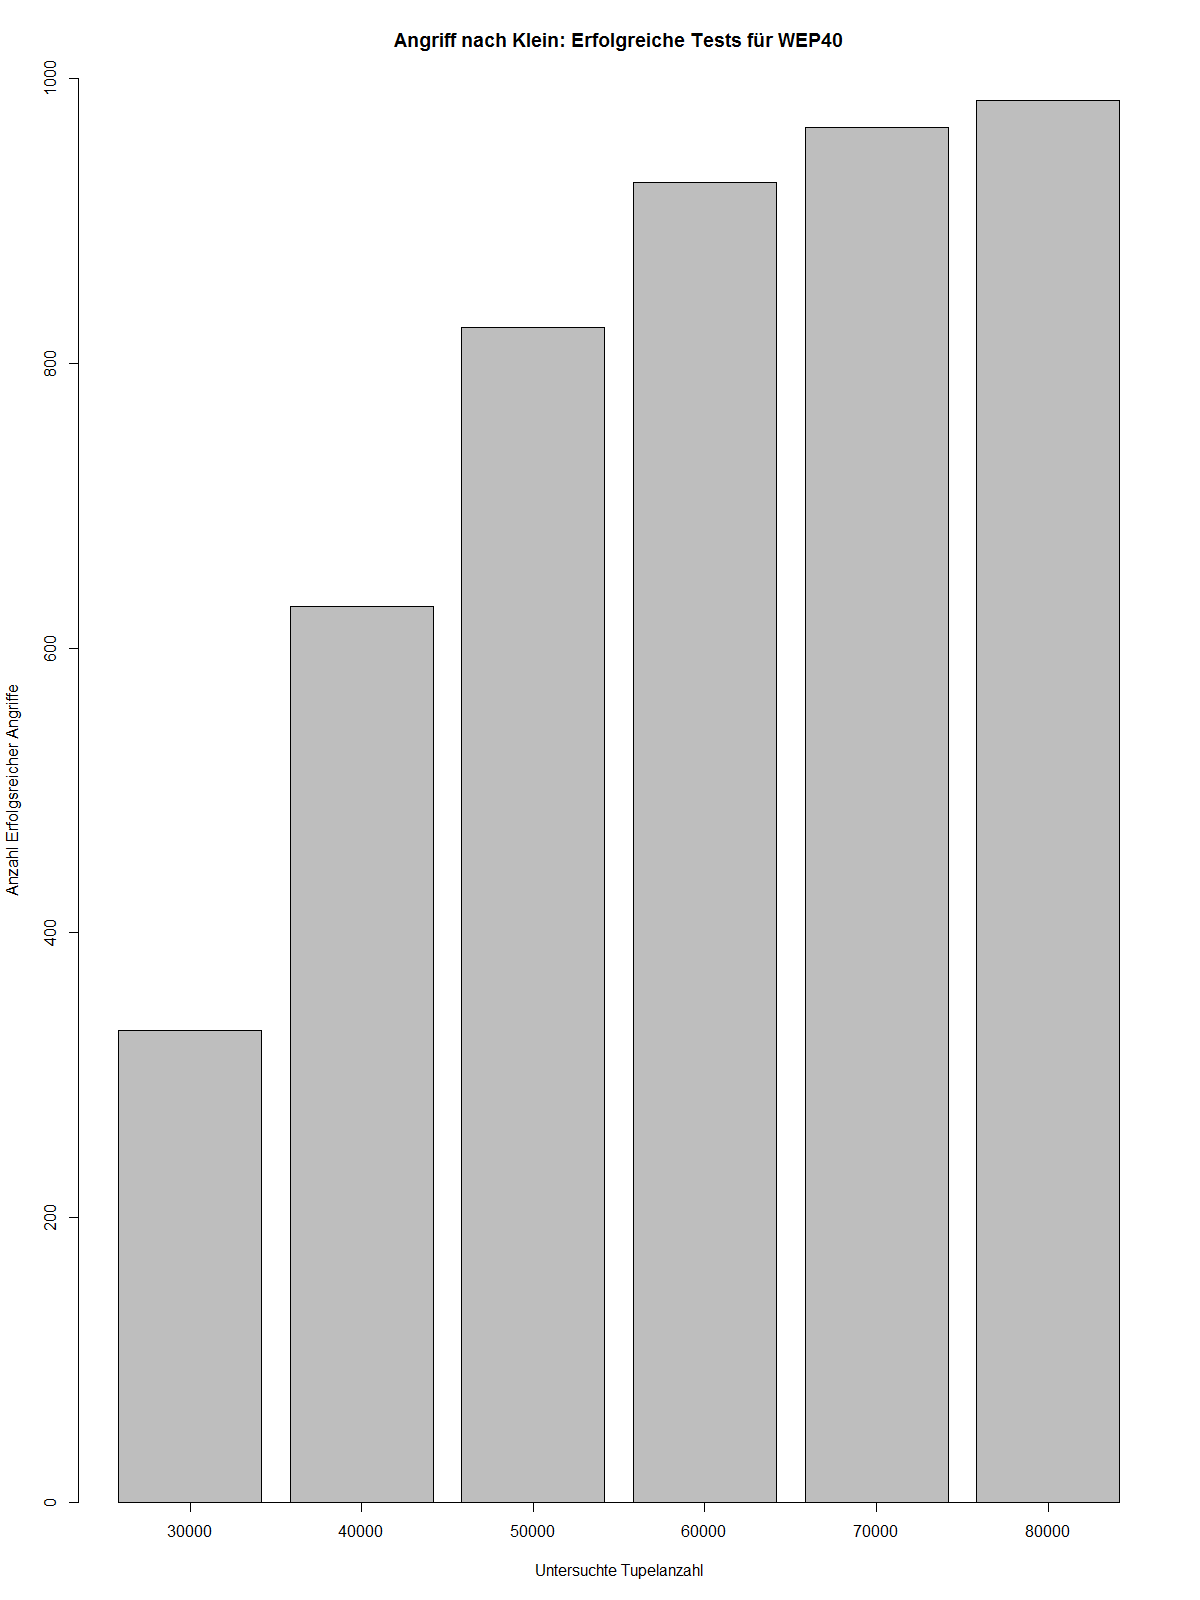
\includegraphics[width=\textwidth]{img/wep40_erfolg.png}
\label{fig:wep40_suc}
\newpage

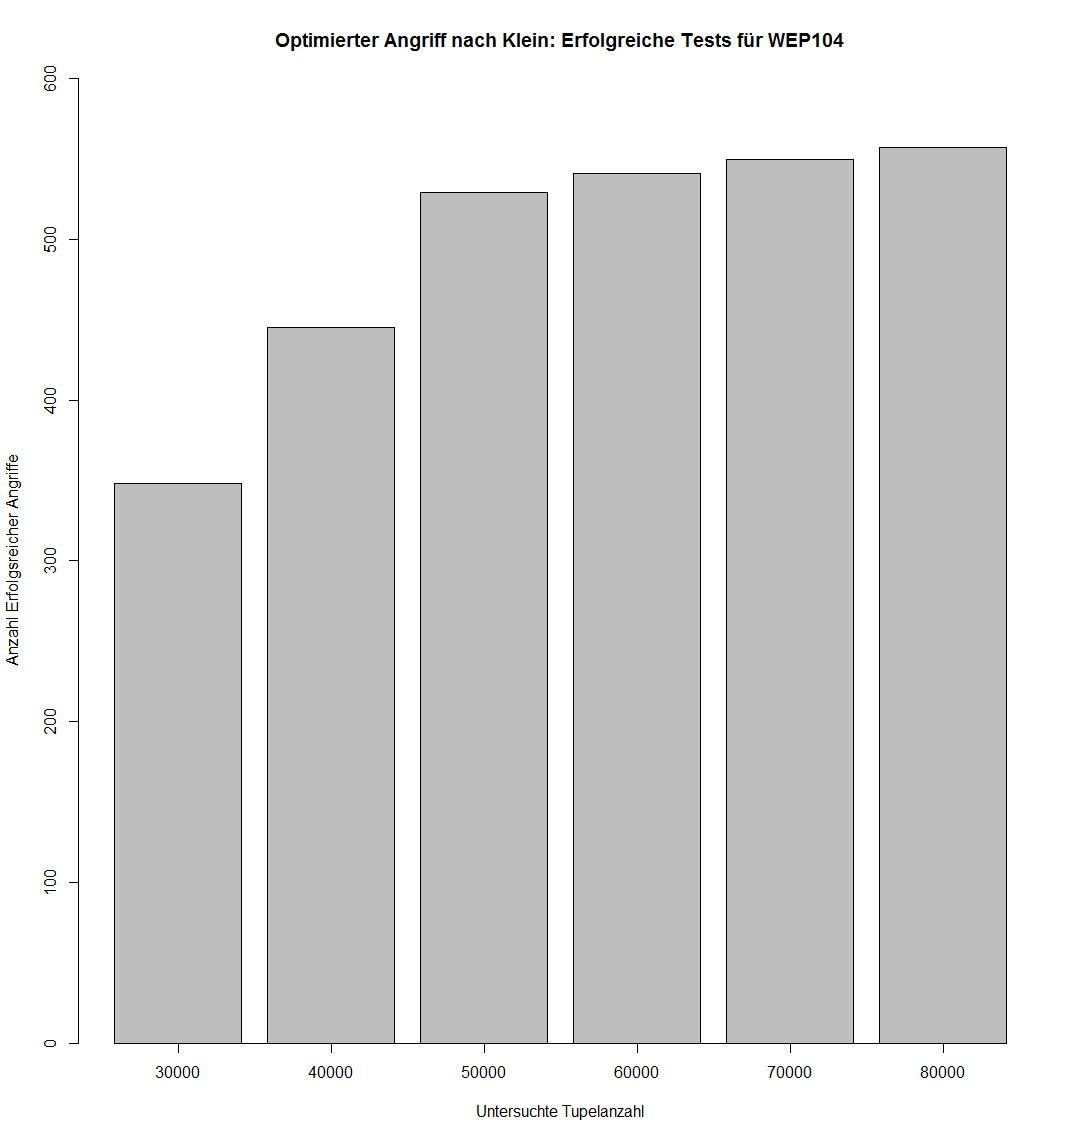
\includegraphics[width=\textwidth]{img/WEP_104_erfolgreich.png}
\label{fig:wep100_suc}
\newpage

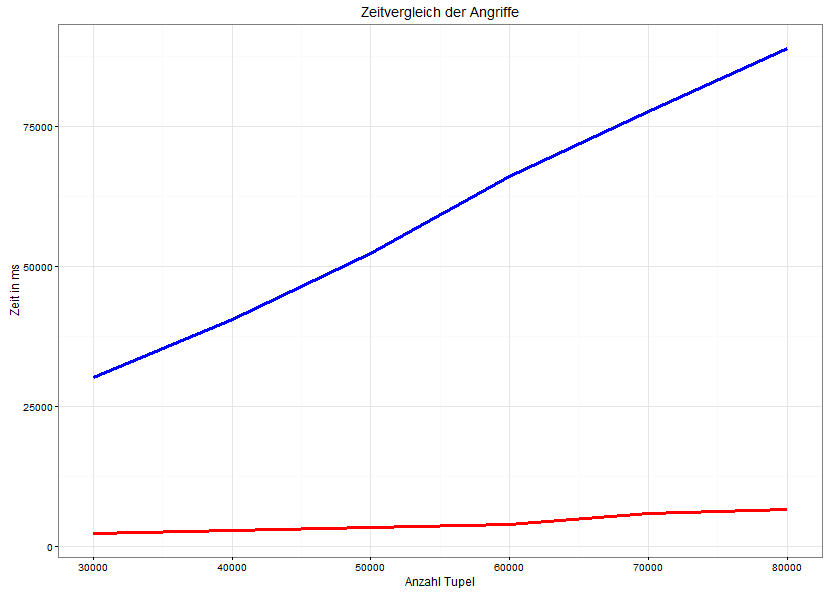
\includegraphics[width=\textwidth]{img/vergleich.png}
\label{fig:vergleich}
\\
Angriff von Klein in blau, Verbesserter Angriff in rot

\newpage

\nocite{*}
\printbibliography
\end{document}
